\title{Final for Calculus-Based Physics: Electricity and Magnetism}
\author{Dr. Jordan Hanson - Whittier College Dept. of Physics and Astronomy}
\date{\today}
\documentclass[10pt]{article}
\usepackage[a4paper, total={18cm, 27cm}]{geometry}
\usepackage{outlines}
\usepackage{graphicx}
\usepackage{amsmath}
\begin{document}
\maketitle

\section{Equations and constants}

\begin{enumerate}
\item Volume of a sphere: $V_s = \frac{4}{3}\pi r^3$.
\item Density, mass and volume: $m = \rho V$.
\item Charge density, charge and volume: $Q = \rho V$.
\item Coulomb force: $\vec{F}_C = k \frac{q_1 q_2}{r^2}\hat{r}$.
\item Centripetal force: $\vec{F} = \frac{mv^2}{r}$
\item Definition of electric field: $\vec{F}_C = q\vec{E}$.
\item Voltage and electric field, one dimension, uniform field: $|E| = - \frac{\Delta V}{\Delta x}$.
\item Charge and capacitance: $Q = CV$.
\item Parallel plate capacitor: $C = \frac{\epsilon_0 A}{d}$.
\item Ohm's Law: $V = IR$.
\item Electrical power: $P = IV = I^2 R = V^2/R$.
\item Magnetic dipole moment: $\vec{\mu} = I \vec{A}$, where $\vec{A}$ is the area vector. $\mu = N I A$ if there are $N$ loops.
\item Torque on a magnetic dipole: $\tau = \vec{\mu} \times \vec{B}$.  The magnitude is $\tau = \mu B \sin(\theta)$.
\item Hall voltage: $emf = B l v$.
\item Definition of magnetic flux: $\phi_m = \vec{B} \cdot \vec{A}$.  The units are T m$^2$, which is called a Weber, or Wb.
\item Faraday's Law: $emf = -N \frac{\Delta \phi}{\Delta t}$.
\item Faraday's Law using \textbf{Inductance}, M: $emf = -M \frac{\Delta I}{\Delta t}$.
\item Typically, we refer to \textit{mutual inductance} between two objects as $M$, and \textit{self inductance} as $L$.
\item Magnetic permeability: $\mu_0 = 4\pi \times 10^{-7}$ T m A$^{-1}$
\item Units of inductance: V s A$^{-1}$, which is called a Henry, or H.
\item Coulomb constant: $k = 8.9876 \times 10^{9}$ N m$^2$ C$^{-2}$.
\item Fundamental charge: $q_e = 1.602 \times 10^{-19}$ C.
\item Speed of light: $\approx 3 \times 10^{8}$ m/s.
\item Permittivity of free space: $\epsilon_0 = 8.85 \times 10^{-12}$ N$^{-1}$ C$^2$ m$^{-2}$.
\end{enumerate}

\clearpage

\section{Exercises}

\begin{enumerate}
\item \textbf{Chapter 18: Electrostatics}
\begin{enumerate}
\item Two charges 3 $\mu$C and 12 $\mu$C are fixed 1 m apart, with the second one to the right. Find the magnitude and direction of the net force on a -2 nC charge when placed at the following locations: (a) halfway between the two (b) half a meter to the left of the left charge. \\ \\
a) 0.6 mN to the right.  b) 0.312 mN to the right. \\
\item A 1 nC charge is fixed at the origin, and a -1 nC charge orbits it at a distance of 1 nm.  (a) What is the Coulomb force between them?  (b) At what speed is the negative charge required to move if the centripetal force balances the Coulomb force, and it has a mass of $10^{-12}$ kg?  How does this speed compare to the speed of light? \\ \\
(a) The Coulomb force is
\begin{equation}
F_c = k\frac{q_1 q_2}{r^2} = 9\times 10^{9} \frac{-1^2 \times 10^{-18}}{(10^{-9})^2} = -9\times 10^{9-18+18}=-9\times 10^{9}~~N
\end{equation}
(b) Set the magnitude of the centripetal force equal to the magnitude Coulomb force:
\begin{align}
F_C &= \frac{m v^2}{r} \\
\sqrt{\frac{r F_C}{m}} &= v = \sqrt{\frac{10^{-9} \times 9 \times 10^{9}}{10^{-12}}} = 3 \times 10^6 ~~ m/s\\
\end{align}
This is one percent of the speed of light. \\
\end{enumerate}
\item \textbf{Chapter 19: Voltage and Capacitance}
\begin{enumerate}
\item The voltage across a capacitor is 100 mV, and the distance between the two charged surfaces is 1 mm.  What is the electric field in the capacitor? \\ \\
When the electric field is uniform, the field is given by the voltage divided by the distance: $E = \Delta V / \Delta x = 0.1/10^{-3}$ V/m, or 100 V/m. \\
\item A parallel plate capacitor has an area of $25 \times 10^{-6}$ m$^2$, and a plate separation of $d = 10^{-4}$ m.  (a) What is the capacitance? (b) What is the total capacitance if two such capacitors are connected \textit{in series}? (c) \textit{In parallel}? \\ \\
(a) The capacitance is $C = 8.85 \times 10^{-12} \times 25 \times 10^{-6} \times 10^{4} = 8.85\times 12 \times 10^{-14} = 1.06$ pF.  (b) The rule for identical capacitors in series is that the capacitance drops by a factor of 2, so $C \approx 0.501$ pF.  (c) Parallel capacitors add, so $2.12$ pF.
\end{enumerate}
\item \textbf{Chapters 20-21: Current, Resistance, and DC Circuits}
\begin{enumerate}
\item Two resistors are connected in series.  One has 1000$\Omega$ resistance, and the other has 500$\Omega$ resistance.  If the resistors are connected in series to a 1.5 V battery, (a) what current will flow? (b) Draw a graph of $I$ vs. $V$ in this system, as if $V$ could vary but the total resistance were fixed.  Label the axes of the graph and indicate the slope. \\ \\
The total resistance is 1500$\Omega$, because the resistors are in series.  Using Ohm's law, we have 1.5V/1500$\Omega$ = 1.0 mA.  The graph is a linear graph, and if we place Volts on the y-axis, and current on the x-axis, the slope will be 1500.  However, if we put current on the y-axis and volts on the x-axis, the slope will be 1/1500. \\
\item How much energy in kiloWatt hours does a $10\Omega$ light consume if it draws 1.0 Amp of current for 6 hours? \\ \\
The relevant equation is $P=IV = I^2 R$.  We have the current and the resistance, so this is a $1.0^2 \times 10.0 = 10.0$ W light bulb.  Thus, a 10W light running for 6 hours consumes 60 W hours of energy, or 0.06 kW hours.  Remember that energy $U = P \Delta t$, so a ``Watt hour'' or ``kW hour'' is an energy, not a power. \\
\begin{figure}
\centering
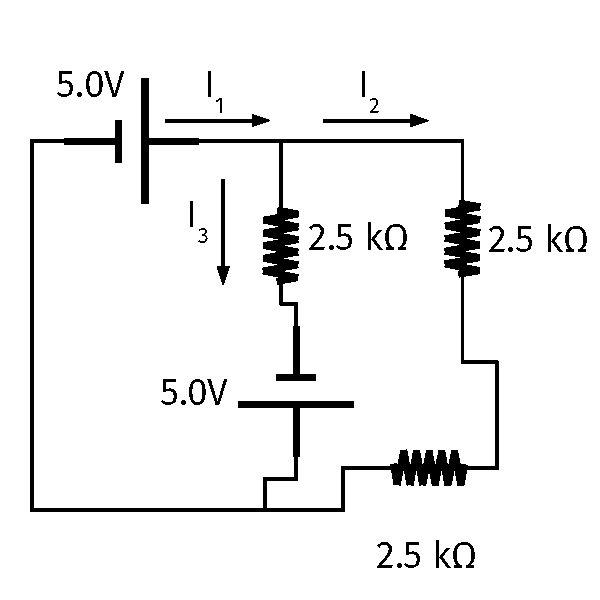
\includegraphics[width=0.3\textwidth]{iV2.pdf}
\caption{\label{fig:batt1} A circuit with two battery voltages and three resistors.}
\end{figure}
\item Solve for the currents in Fig. \ref{fig:batt1}.
\begin{itemize}
\item $I_1 = 5$ mA
\item $I_2 = 1$ mA
\item $I_3 = 4$ mA
\end{itemize}
\end{enumerate}
\item \textbf{Chapter 22: Magnetism}
\begin{enumerate}
\item A Hall effect flow probe is placed on an artery, applying a 0.1 T magnetic field across it. What is the blood velocity, given the vessel’s inside diameter is 4.00 mm and the Hall voltage is 0.8$\mu$V? \\ \\
The Hall effect follows $emf = B l v$, or $v = emf / (B l) = 0.8 \times 10^{-6} / (0.1 \times 4 \times 10^{-3}) = 2$ mV. \\
\item A circular loop of wire of area $10^{-1}$ m$^{2}$ carries a current of 1.0 A, and it is situated in the xy plane.  (a) An external 1.0 T B-field is applied in the positive z-direction.  What is the magnitude of the torque? (b) A magnetic field is applied in the x-direction.  What is the magnitude of the torque? \\ \\
(a) In the first case, the magnetic moment of the loop is in the +z direction, and so is the field, so the torque is zero.  (b) $|\vec{\tau}_m| = |\vec{\mu} \times \vec{B}| = \mu B\sin(\theta)$.  The angle is 90 degrees, so the torque is $\mu B = I A B = 1.0\times 10^{-1} \times 1.0 = 10^{-1}$ N m.
\end{enumerate}
\item \textbf{Chapter 23: Electromagnetic Induction and Inductance}
\begin{enumerate}
\item Suppose we encounter two inductors and decide to measure the inductance of each.  One is smaller, producing an emf of $5$ mV if the current across it is changed at a rate of 50 A/s.  The larger produces an emf of $10$ mV for a rate of 50 A/s.  What is the inductance of each? \\ \\
(a) The smaller inductance is $L = emf/(\Delta I/\Delta t) = 5 \times 10^{-3}/50 = 0.1$ mH.  Using scaling, we conclude that the second inductor is $0.2$ mH. \\
\item Suppose the two inductors were interleved, such that a current through one inductor would generate a solenoidal magnetic field that happened to pass through the other solenoid.  If a changing current is passed through the smaller inductor, which of the following is true of the larger?
\begin{itemize}
\item A: Nothing would happen: the emf is only induced in the first inductor.
\item B: An emf would be induced in the second inductor, equal to the emf in the first inductor.
\item C: An emf would be induced in the second inductor, but smaller than the emf in the first inductor.
\item D: An emf would be induced in the second inductor, but larger than the emf in the first inductor.
\end{itemize}
\textit{The answer is D, because the larger inductor sees the same flux as the smaller, but with more coils.  Thus, the induced emf is larger in the larger inductor.}
\end{enumerate}
\item Camera flashes charge a capacitor to high voltage by switching the current through an inductor on and off rapidly. In what time must the 0.100 A current through a 2.00 mH inductor be switched on or off to induce a 500 V emf? \\ \\
Use $|emf| = L \frac{\Delta I}{\Delta t}$.  Solve for $\Delta t = L \frac{\Delta I}{emf} = 2 \times 10^{-3} \frac{0.1}{5 \times 10^{2}} = \frac{2}{5} \times 10^{-6} = 0.4 \mu$s.
\end{enumerate}

\end{document}